%EP 1 de Laboratório de Simulação e Computação
%Aluno: Daniel Oliveira Caires
%Numero USP: 5197211
%Curso: Bacharelado em Matemática Aplicada e Computacional
%Turma 54 - Período Noturno

\documentclass[a4paper,12pt]{article} 
\usepackage[brazil]{babel}
\usepackage[utf8]{inputenc} 
\usepackage{amsmath}
\usepackage{amssymb}
\usepackage{graphicx}

\title{Laboratorio de Simulação e Computação - Trabalho 1}
\author{Daniel Caires}
\date{}

\begin{document}
\maketitle

	Não é incomum que meus amigos estranhem quando digo que há disciplinas de computação no curso de matemática, e é curioso pensar que a relação entre ambas não seja clara para pessoas que não sejam da área. Pois qual serã a importância da matemática para a computação e vice-versa?

	\section{A computação e a Matemática}
		Programas de computador são escritos como uma série de instruções lógicas e matemáticas. O primeiro programa de computador foi escrito pela matemática inglesa do século $XIX$ Ada Lovelace.\\
		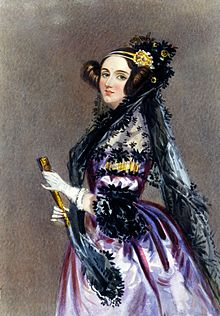
\includegraphics[scale=0.5]{ada.jpg}

		Além da estrutura matemática que é intrínceca da programação, a computação é fundamental para a solução de problemas matemáticos de grande complexidade. Computadores são capazes de executar muitas operãções matemáticas em um curto tempo, sendo assim, problemas matemáticos que que requeiram uma grande quantidade de cálculos eram inviáveis antes da computação.\\

		Entre esses tipos de problemas, podemos usar como exemplo as técnicas de integração numérica. Que tem como objetivo aproximar o valor de integrais definidas sem o uso de suas primitivas, um de seus métodos básicos é a chamada quadratura numérica que consisete na seguinte expressão:
		\begin{equation*}
			\int_a^b f(x)dx \approx \sum_{i=0}^n \alpha_i f(x_i)
		\end{equation*}


	\section{O curso de Simulação e Computação}
		Esntre os problemas matemáticos complexos que necessitam de métodos computacionais para serem resolvidos, destacam-se os problemas de simulação computacional.\\
		
		Através da siulação de variáveis aleatórias de diferentes tipos de distribuição. Podemos simular modelos complexos de problemas reais e estudar seu comportamento sob diversas condições. O curso Laboratório de Simulação e Computação vai nos fornecer as ferramentas necessárias para estudar, modelar e solucionar esses tipos de problemas complexos.
		

%	\begin{thebibliography}{3}
%		\bibitem[Ada Lovelace - Wikipedia]{wikipedia}
%		https://en.wikipedia.org/wiki/Ada_Lovelace
%		\bibitem[Jupiterweb - Programa da Disciplina de MAP2212]{jupiterweb}
%		https://uspdigital.usp.br/jupiterweb/obterDisciplina?sgldis=MAP2212&codcur=45070&codhab=4
%		\bibitem[Numberphile]{numberphile}
%		http://www.numberphile.com
%	\end{thebibliography}

\end{document}
